\documentclass[11pt, a4paper, hyphens]{article}
\usepackage[a4paper, left=30mm, right=30mm]{geometry} % margin=2.6cm

\usepackage[utf8]{inputenc}  % allow utf-8 input
\usepackage[T1]{fontenc}     % use 8-bit T1 fonts
\usepackage{ebgaramond}

\usepackage{hyperref}         % hyperlinks
\usepackage{url}              % simple URL typesetting
\usepackage{booktabs}         % professional-quality tables
\usepackage{amsfonts}         % blackboard math symbols
\usepackage{nicefrac}         % compact symbols for 1/2, etc.
\usepackage{microtype}        % microtypography
\usepackage{xcolor}           % colors
\usepackage{bbm}
\usepackage{amsthm}
\usepackage{rotating}
\usepackage{pdfpages}

\hypersetup{                 % setup the hyperref package
    colorlinks=true,
    linkcolor=blue,
    filecolor=blue,
    urlcolor=blue,
    citecolor=blue,
    pdftitle={Entitlement Justice and Measures of Algorithmic Fairness},
    pdfauthor={Edward Speer, Llama-2-7b},
    pdfkeywords={entitlement justice, algorithmic fairness, AI ethics},
    bookmarks=true,
}

\usepackage{graphicx} % Required for inserting images
\usepackage[ngerman, english]{babel}
\usepackage[iso, ngerman]{isodate}


\usepackage{bbold}
\usepackage{mathtools}
\usepackage{amsmath} % Required for \DeclareMathOperator
\usepackage{nicefrac}
\usepackage{tikz}
\usepackage{subcaption}
\usepackage{centernot} % for the comparison

%\theoremstyle{definition}
\newtheorem{definition}{Definition}
\newtheorem{theorem}{Theorem}

\usepackage{verbatim}

\RequirePackage[T1]{fontenc} 
\RequirePackage[tt=false, type1=true]{libertine} 
\RequirePackage[varqu]{zi4} 
\RequirePackage[libertine]{newtxmath}

\usepackage[round,comma]{natbib}
\bibliographystyle{plainnat}

\newcommand{\monthyeardate}{\ifcase \month \or January\or February\or March\or %
April\or May \or June\or July\or August\or September\or October\or November\or %
December\fi, \number \year} 

\title{The Role of Large Language Models in Academic Writing}
\author{%
  Edward Speer
  \\
  California Institute of Technology\\
  \texttt{espeer@caltech.edu} \\
}
\date{\monthyeardate}

\begin{document}

\maketitle

\section{Introduction}\label{sec:introduction}

The majority of research journals now provide policies for the use of large
language models (LLMs) in academic writing. In the Nature journals, for example,
``Large Language Models do not satisfy our authorship criteria. Notably, an
attribution of authorship carries with it accountability for the work, which
cannot be effectively applied to LLMs''~\citep{nature_ai_policies}. For Cambridge
Press, ``AI does not meet the Cambridge requirements for authorship, given the
need for accountability''~\citep{cambridge_ai_policies}. The chief concern among
these policies appears to be responsibility. The policies don't outright ban the
use of AI, nor do the outline specific guidelines for how to appropriately use
LLMs, save for as a copy-editor, but they make specific prohibitions against
authorship and attribution of writing to LLMs. It seems clear that the journals
are targeting issues of accountability. Who should the journal turn to when a
mistake is discovered in a paper? Who is the owner and originator of the ideas
presented? Who should be legally liable for the content of the paper? 

The policies are clear that human authors alone must take
full responsibility for the content of their papers, and to that end, LLMs
cannot be considered coauthors. The need for accountability goes beyond concerns
about liability for errors in writing, however, The policies also reflect a
concern about the ownership of ideas and plagiarism. LLMs are trained on vast 
amounts of text, and it is not always clear how to attribute information they
produce. An LLM may produce information that is similar or identical to text in
its training data without a citation, and if this text is included in a paper,
it constitutes plagiarism. The emphasis on accountability in these policies
implies that in this situation, the human authors of the paper would be held
liable for the plagiarism, even if they were unaware of it.

The policies protect the journals from liability in the case of these plagiarism
concerns, but they are largely predicated on the idea that LLMs are not capable
of originating novel ideas of their own. The policies are clear that LLMs cannot
be attributed authorship, meaning that if they did produce original arguments,
authors would be faced with a choice of either not publishing those ideas 
(stifling potentially significant contributions to the field) or not properly
attributing them, neither of which is a desirable outcome. This means that
should we find LLMs capable of producing original ideas, the current policies
are out of step with the capabilities of the technology and require rapid 
revision. Even if LLMs do not currently have this ability, it is possible they
could attain them in the near future, and thus these policies are at risk of
quickly becoming out of date. We therefore need to both discover and explore the
capabilities of LLMs in producing new ideas, and to consider the implications
of these capabilities for the future of academic writing.

In this paper, we attempt to explore the ability of a current LLM to contribute
original ideas and argumentation to an original philosophical research paper.
We do this by using an LLM to collaborate on a research paper in the field of
algorithmic fairness and distributive justice. The goal of the project is to
produce a high-quality research paper that constitutes an original contribution
to the field, and in the process, to use the LLM to its fullest potential and
explore the capabilities and limitations of doing so. The goal of this
experiment is not simply to see if the LLM can produce a publishable paper, but
rather to explore the utility of using an LLM in a genuine effort to produce a
high-quality paper. This effort will be a collaborative one, with both the human
author and LLM writing sections of the paper, providing feedback on each other's
writing, suggesting sources, and engaging in discussion about the ideas
presented with the goal of producing the best paper possible. The success of
such an endeavor is difficult to measure; we seek to provide a qualitative
assessment of the LLM's contributions to the paper, and to explore the
implications of the growing capabilities of LLMs for the future of academic
writing. With the ongoing and rapid development of LLMs in mind, this paper is
not meant to be a definitive assessment of the capabilities of LLMs, but rather
an exploration of a specific model's capabilities and limitations as well as a
discussion of the future of academic writing in light of these technologies.

For this project, we chose as the subject of our paper the topic of algorithmic
fairness measures and their connection to the philosophical concept of
distributive justice. Algorithmic fairness measures are a critical component of
the design and deployment of machine learning systems, as they are intended to
ensure that these systems do not discriminate against individuals based on
sensitive attributes. Distributive justice, on the other hand, is a central
concept in political philosophy that concerns the fair distribution of social
goods. Distributive justice exists on a spectrum from end-state theories, which
analyze whether a given distribution of resources is fair, to historical
theories, which analyze whether the history of transactions that led to a given
distribution of resources is fair. Since algorithmic fairness measures are often
used to evaluate the fairness of algorithmic systems that make decisions about
the distribution of resources such as bank loans or job opportunities, there is
a natural connection between these two topics. The relationship between the two
fields has been explored in the literature, but in the early stages of this
project, our LLM suggested that there is a lack of discussion in the literature
about the relationship between algorithmic fairness measures and historical
theories of distributive justice. Our investigation began from this vague notion
of the intersection between the two fields, and we worked with the LLM from this
point to develop and complete a specific research project on the topic.

This paper will be structured as follows. In Section~\ref{sec:methods}, we will
present the methods used, including the specific LLM selected for the
investigation and the program used to interact with it. In
Section~\ref{sec:results}, we will present the full text of the paper produced
in collaboration with the LLM. In Section~\ref{sec:analysis}, we will analyze
the role of the LLM throughout 5 task-stages of the research process: literature
review, research question formulation, argumentation, writing, and revision.
Finally, in Section~\ref{sec:conclusion}, we will conclude with a discussion of
the implications of this experiment for the future of academic writing. Note
that an LLM was only used as a collaborator for the writing of the research
paper presented in Section~\ref{sec:results}, and not for the writing of this
introduction or any other part of the paper. The introduction, analysis, and
discussion outside of Section~\ref{sec:results} were written entirely by the
human author of this paper without the assistance of LLMs.


\section{Methods}\label{sec:methods}

For this experiment, we selected the Llama-2-7b model developed by Meta AI. The
Llama-2-7b model is a large language model trained on a diverse range of
textual data, including books, articles, and websites. The model is capable of
generating coherent and contextually relevant text across a wide range of
domains. We selected this model for its ability to generate high-quality text
and its general-purpose nature, which makes it suitable for a wide range of
writing tasks, as well as for its open source nature, which reflects our
commitment to transparency and reproducibility. While models like GPT-4o are 
continuously updated and improved in inscrutable ways, Llama-2-7b serves as a
stable fixed-point for our investigation.

We engaged with the Llama-2-7b model (henceforth referred to as Llama) using a
web-hosted API called Llama-api (\url{https://www.llama-api.com/}). This API
allows users to pay a per-token fee to interact with the model via an http
request to a designated endpoint. A user sends a prompt to the model, including
context memory built up over the course of the interaction and the limitations
on response tokens, and the model generates a response based on the prompt and
the context memory.

In order to manage the use of Llama, we built a custom chat application in
Python that allowed us to communicate with the model from the command line.
This application has the following features:
\begin{itemize}
    \item \textbf{Chat logging}: User prompts and responses from Llama are
    automatically saved to a log file in markdown format for future analysis.
    \item \textbf{Context Memory Management}: The application allows the user
    to save and use different streams of context memory across different
    sessions with the model. For example, in the beginning of one context, Llama
    is told ``I am a philosopher and computer scientist. You are my co-author.
    We are writing a philosophy paper. We are focused on measures of algorithmic
    fairness and the concept of justice they enforce.'' In another context,
    Llama can be told to act as a reviewer, or to speak in the voice of an
    author encountered in the literature review. These bits of context are saved
    in compressed pickle files and can be loaded into the application at the
    any time during a session.
    \item \textbf{Manual Context Editing}: The application allows the user to
    manually edit the context memory before sending it to Llama. This is useful
    for trimming down the context memory to the most relevant information to
    reduce the cost of the interaction and to focus the model on critical
    information. This feature can also be used to pass entire papers or large
    sections of text to Llama for review or comment.
    \item \textbf{Token Limiting}: The application allows the user to set a
    limit on the number of tokens in the response from Llama. This is useful for
    managing the cost of the interaction with the model.
\end{itemize}
The full source code for the chat application is accessible
from~\ref{sec:appendixI}.

Three main threads of context memory were used to work with Llama in this study.
In the first thread, Llama was presented with the true circumstances of the
experiment: that it was acting as a co-author on a philosophy paper about
algorithmic fairness measures and distributive justice. In the second thread,
Llama was presented with the role of a reviewer of the paper, providing feedback
on the argumentation and writing. In the third thread, Llama was not prompted
with any particular role, but was simply continually asked to explain particular
arguments or concepts from the literature with appropriate citations. Henceforth
we will refer to these roles as the coauthor, reviewer, and explainer roles. 
Each of these roles was used throughout the research and writing process, with
the exception of the reviewer role which was used only during revision. The full
logs of interactions with the model including which context memory was used in
each interaction are available in~\ref{sec:appendixI}.

Co-authorship is a relationship which can take on many forms depending on the
nature of the collaboration. In this case, we were interested in exploring the
extent to which Llama could contribute substantive and original content. This
goal determined the nature of the interactions with Llama, which were designed
to elicit original ideas and argumentation from the model. Simply asking the
model to write the paper or to produce large sections of the text would not have
been a useful approach — anyone who has asked an LLM to do so is aware that the
results are lacking in depth or originality. Instead, in each of the five tasks
of the research process, we engaged Llama in structured dialogues that
contributed to the development of the paper. The structure of this dialogue was
inspired by the Socratic method, and proceeded in a set of steps:
\begin{enumerate}
    \item Provide Llama with the relevant background knowledge to the discussion
          through the context memory mechanism, pasting relevant sections of
          text, or asking Llama to summarize relevant arguments to add them to
          the context memory. For example, asking ``Please summarize the paper
          `Procedural Versus Substantive Justice: Rawls and Nozick' by David
          Lewis Schaefer'' will add a (Llama generated) summary of the paper to
          the context memory.
    \item Ask Llama a fully open-ended question about the topic at hand. For
          example, ``Tell me about how these fairness measures may emphasize
          distributive concepts of justice?''
    \item Pick out interesting aspects of Llama's response, and ask for more
          detail. For example, ``I found interesting what you said about
          counterfactual measures of algorithmic fairness. How could they be
          considered to emphasize individualized justice in a way that touches
          on entitlement?'' Push on these responses until Llama is unable to
          provide more detail in a coherent way. ``I'm missing some of your
          ideas. In entitlement justice, we focus on whether individuals who
          acquire holdings are entitled to those holdings. Can you explain how
          counterfactual measures of justice show this feature?''
    \item Inject some of your own thoughts into the conversation and ask Llama 
          to respond to them and incorporate them into its own analysis. ``If we
          want to say that someone is entitled to their college admissions, we
          need to say it is their property which is being taken away if they are
          denied admissions. This means that admission is a property acquired
          through work before applying. How should we defend this perspective?''
\end{enumerate}

This dialogue structure is meant to do three things. Firstly, provide Llama with
a basic set of text to pull structures from and hopefully build on. Secondly,
try to draw out original ideas from Llama by really pushing it to do more than 
spit out responses to in-dataset prompts by asking for more details and
explanations than would be found in the training data. Thirdly, to provide some
original text to Llama from outside of the training set to help it build on and
hopefully produce original ideas. Illustrative examples of this interaction and
responses provided by Llama are provided in the analysis section. In a way the
goal was to cause Llama to ``hallucinate'' original ideas by pushing it to build
on its own responses and to build on original text provided by the user.


\section{Results}\label{sec:results}

What follows is the full text of the paper produced in collaboration with Llama.

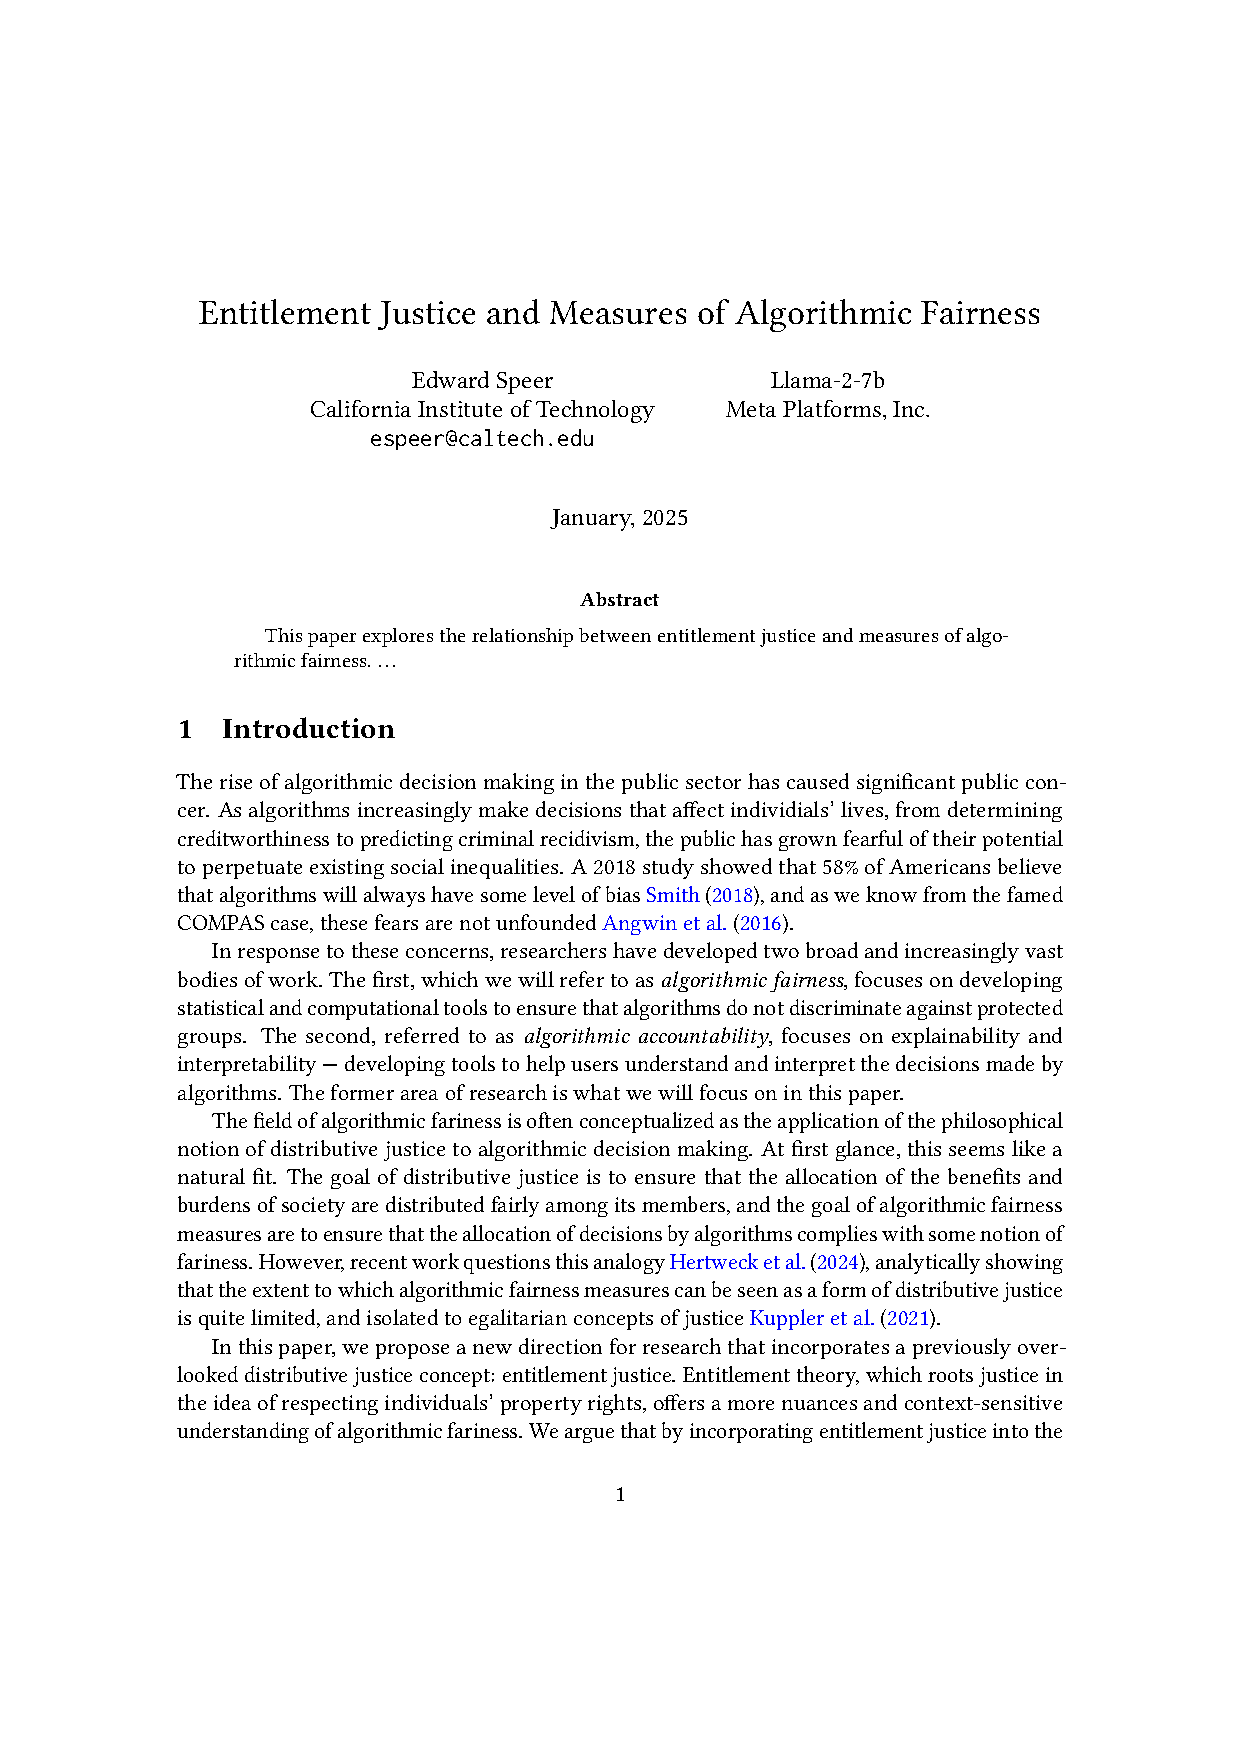
\includepdf[pages=-]{../src/top-level.pdf}

\section{Analysis}\label{sec:analysis}

\section{Conclusion}\label{sec:conclusion}

\section{Appendix I}\label{sec:appendixI}

The full source code for the chat application used in this study as well as all
chat logs are available at the following link: 
\url{https://github.com/Espeer5/paperInAPaper}

% \bibliography{references}
\end{document}